

%\begin{figure}
%	\centering
%   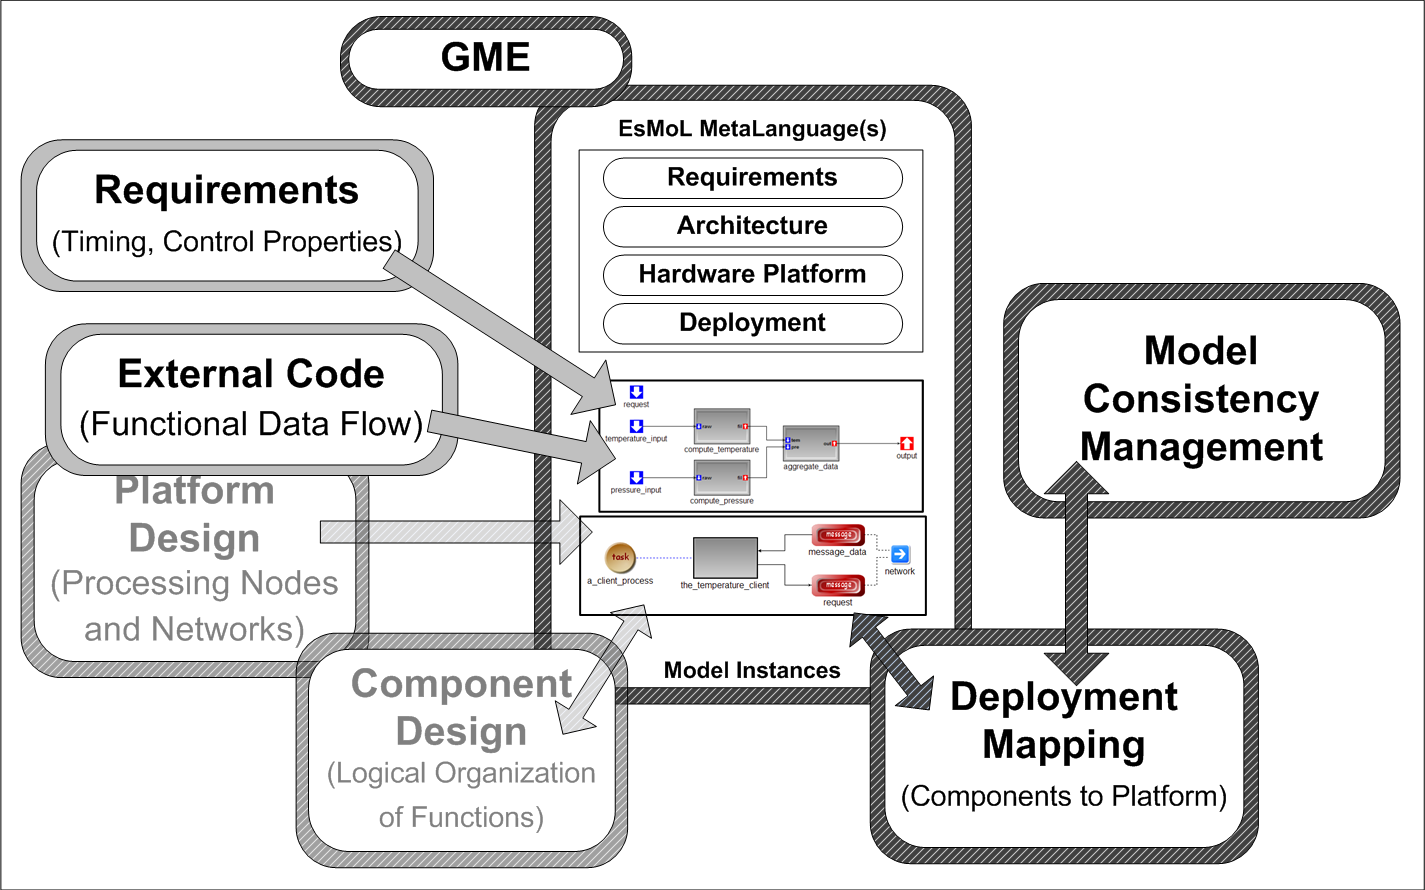
\includegraphics[width=0.55\columnwidth]{diagrams/usecase3.png}
%   \caption{equirements modeling and automated management of deployment models when functional and platform models change.  }
%   \label{fig:uc3}
%\end{figure}

%Fig. \ref{fig:uc3} depicts features of designs in progress.  
Many types of requirements apply to real-time embedded control systems design. Embedded systems are heterogeneous, so requirements can include constraints on control performance, computational resources, mechanical design, and reliability, to name a few things. Formal safety standards (e.g. DO-178B~\cite{DO178B}) impose constraints on the designs as well as on the development process itself.  Accordingly, current research has produced many techniques for formalizing requirements (e.g. ground models in abstract state machines~\cite{Borger} or Z notation~\cite{Z2}).  Models could be used to incorporate formal requirements into other aspects of the design process.  During analysis, requirements may appear as constraints in synthesized optimization problems or conditions for model checking.  Requirements can also be used for test generation and assessment of results.

Management of model updates is also essential. As designs evolve engineers and developers reassess and make modifications.  Changes to either the platform model or functional aspects of the design may invalidate architecture and deployment models created earlier.  Some portions of the dependent models will survive changes.  Other parts needing changes must be identified.  Where possible, updates should be automated.

\subsection{Integration Details}

\begin{figure}
	\begin{minipage}{2.25in}
	\centering
   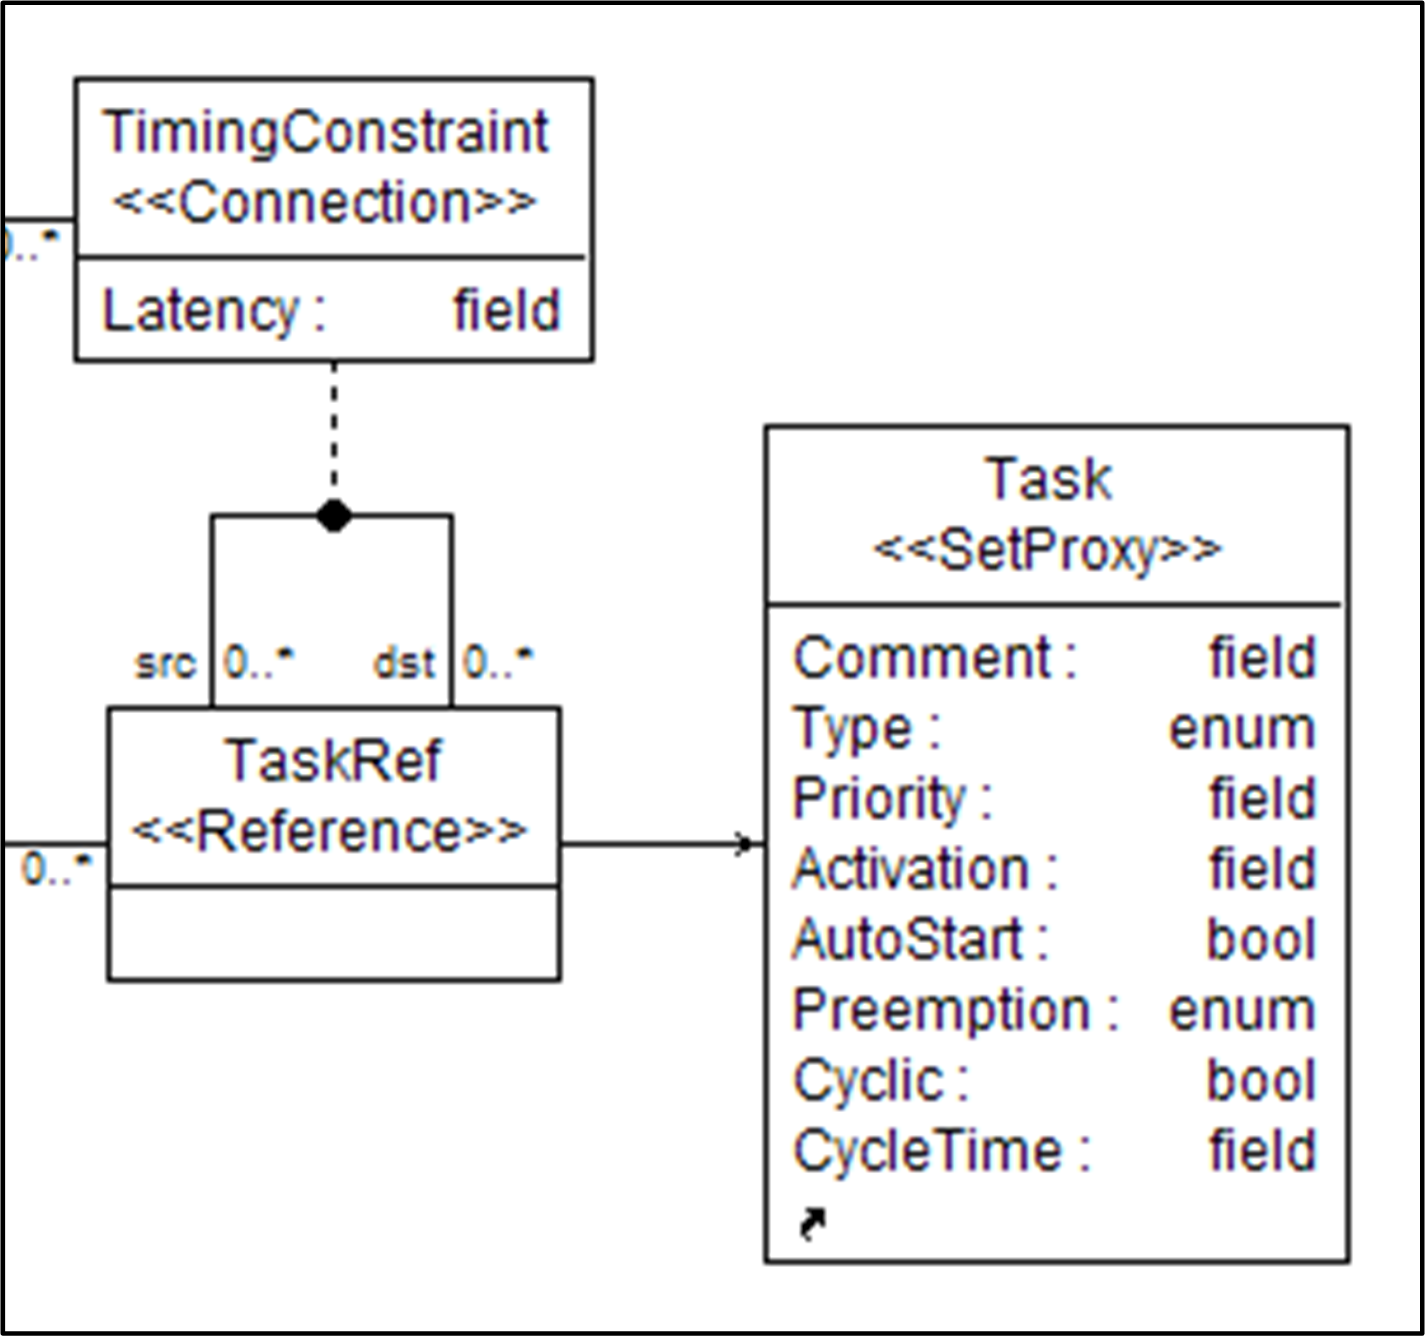
\includegraphics[width=0.75\columnwidth]{diagrams/reqs.png}
   \caption{Latencies are timing constraints between task execution times. }
   \label{fig:reqs}
\end{minipage}
\hspace{0.125in}
	\begin{minipage}{2.375in}
	\centering
   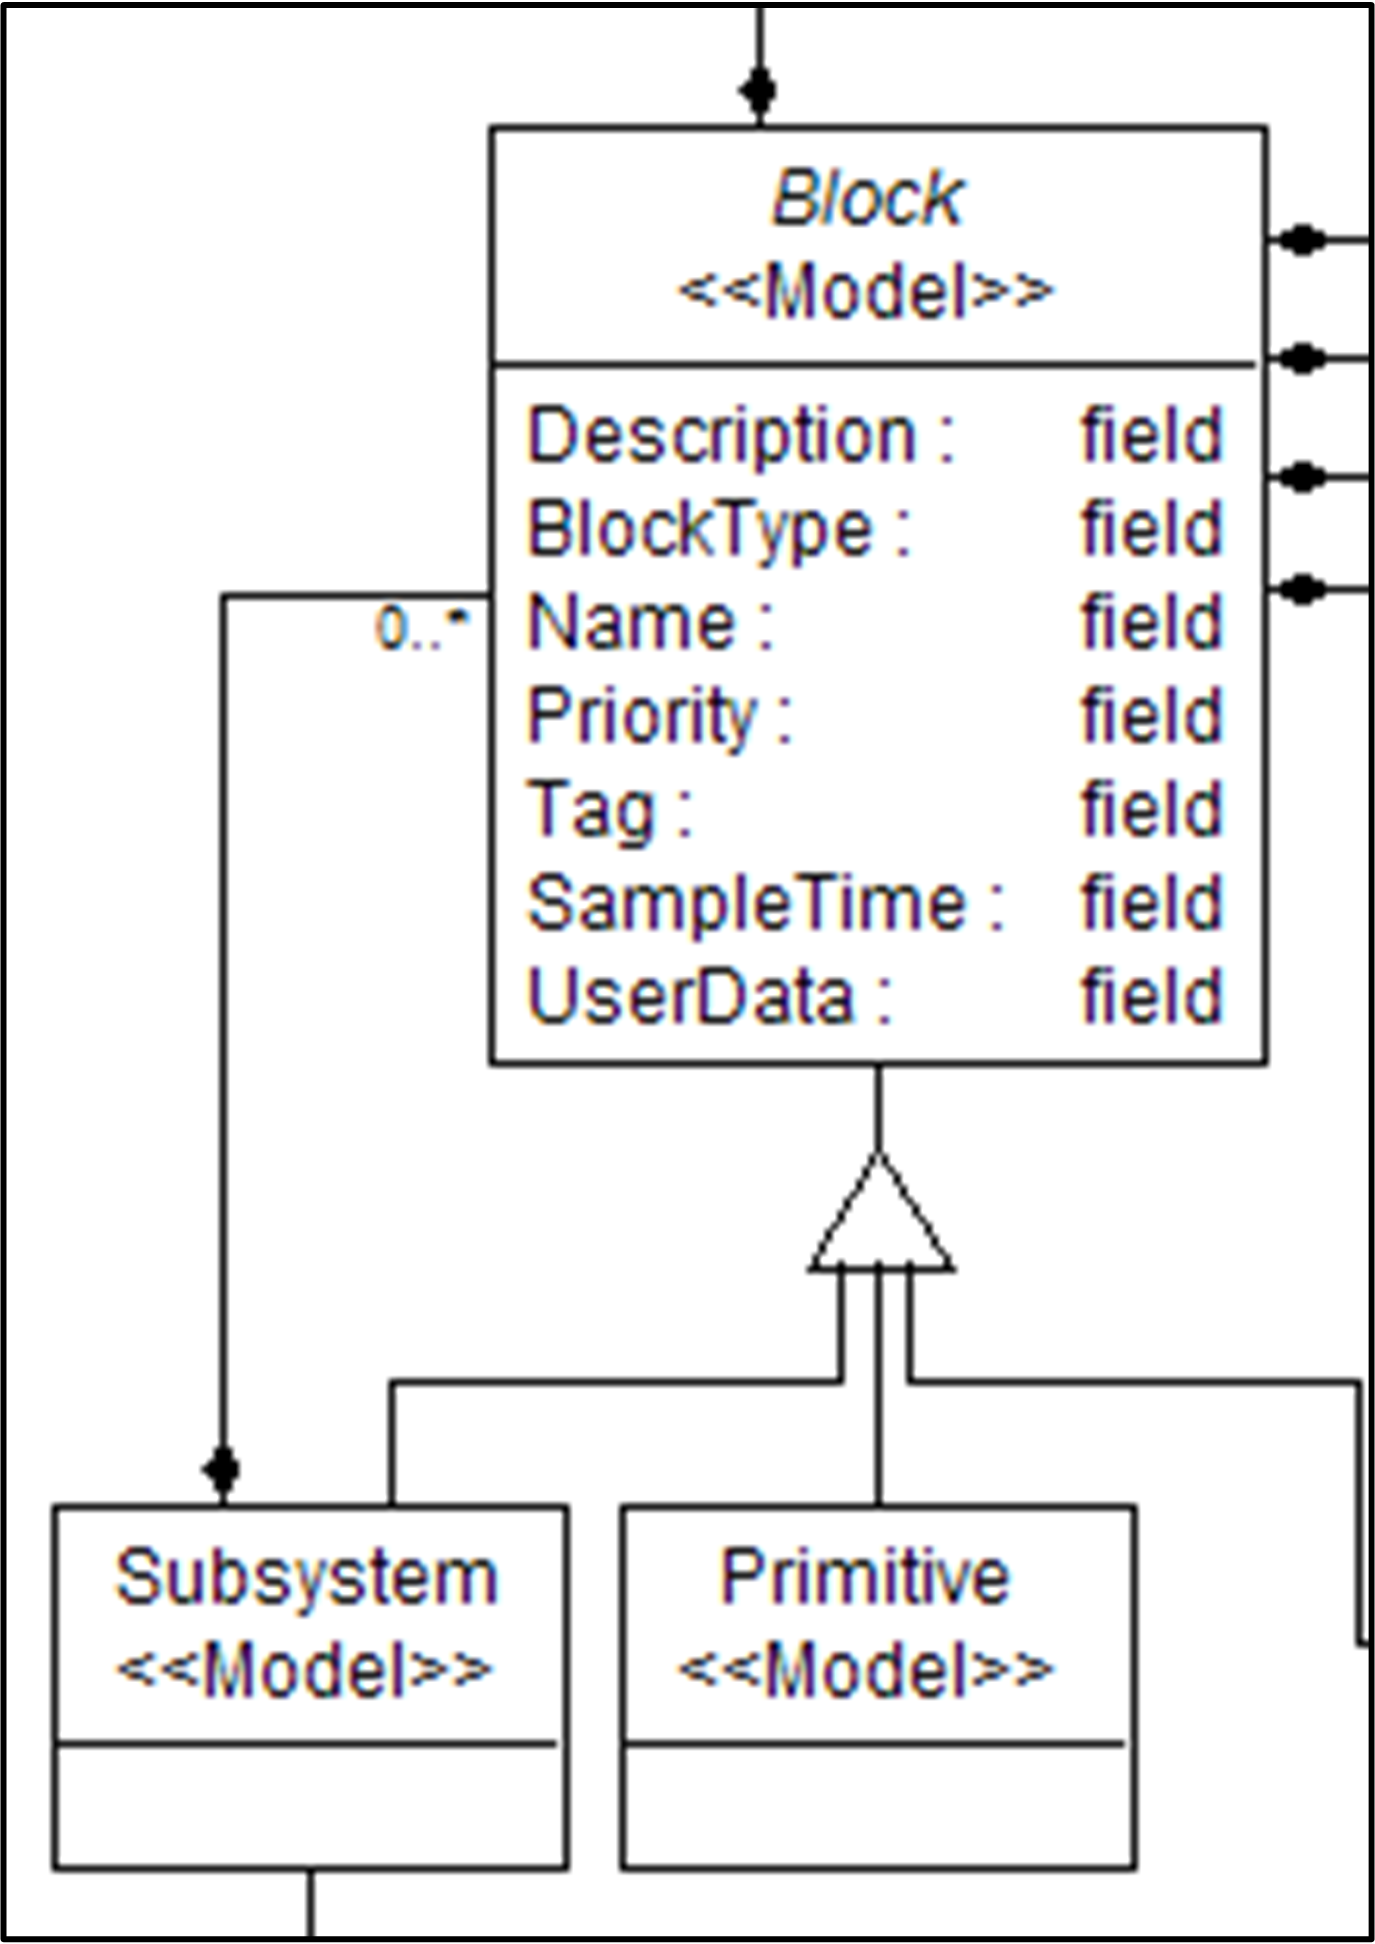
\includegraphics[width=0.65\columnwidth]{diagrams/userdata.png}
   \caption{Simulink's UserData field can help manage model changes occuring outside the design environment. }
   \label{fig:userdata}
   \end{minipage}
\end{figure}

The requirements sublanguage is in design, and so is light on details. Fig. \ref{fig:latency} shows an example model with latency requirements between tasks, and Fig. \ref{fig:reqs} shows the modeling language definition.  This simple relationship can be quantified and passed directly to the schedule solver as a constraint.  Ideally a more sophisticated requirements language could capture the syntax and semantics of an existing formal requirements tool.  Some candidate languages and approaches are currently under consideration for inclusion in the framework.  

\begin{figure}
	\centering
   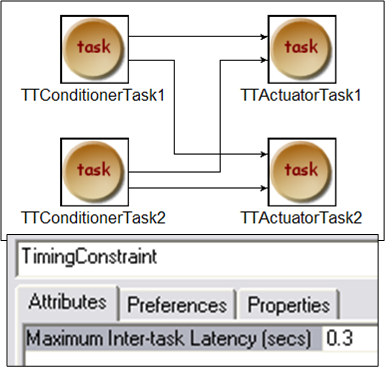
\includegraphics[width=0.55\columnwidth]{diagrams/latency.png}
   \caption{Example of task latency spec for sample model, with detail of timing attribute value specified on model links.}
   \label{fig:latency}
\end{figure}

To track model changes we propose to use the Simulink UserData field to store unique tags when the models are imported.  During an update operation tags in the control design can be compared with previously imported tags in the model environment.  Fig. \ref{fig:userdata} shows the UserData attribute from our Simulink sublanguage, corresponding to the actual attribute in Simulink blocks.  
%Successful updating relies on restriction of the hierarchy.  Allowing the modeling environment to track changes at any depth in the hierarchy can allow some algorithmically difficult situations. With restricted depth lower level details are abstracted away, leaving only changes that would affect the software architecture or deployment relationships.  This imposes some reasonable discipline on control designers, who must organize the top level of their Simulink designs into functional blocks.  Another benefit of this structural requirement is added clarity of designs.
To handle issues arising from topology concerns, we require control designers to group top-level functionality into subsystems and place a few restrictions on model hierarchy in deployment models.

%\subsection{Current and Future Work}

%All of these language elements and features are in the early stages of design or prototype, though work has been done to flesh out many of the required details.